\documentclass[9pt]{beamer}

\usepackage{appendixnumberbeamer}
\usepackage{booktabs}
\usepackage[scale=2]{ccicons}
\usepackage{pgfplots}
\usepackage{tikz}
\usepackage{graphics}

\usepgfplotslibrary{dateplot}
\pdfstringdefDisableCommands{\def\translate#1{#1}}
\geometry{paperwidth=140mm, paperheight=105mm}
\usetheme{metropolis}
\bibliographystyle{abbrv}
\setbeamertemplate{frame footer}{NASA Space Apps Challenge 2024}

\usetikzlibrary{shapes, arrows}
\tikzstyle{startstop} = [rectangle, rounded corners, minimum width=2cm, minimum height=1cm, text centered, draw=black, fill=red!30]
\tikzstyle{io} = [trapezium, trapezium stretches=true, trapezium left angle=70, trapezium right angle=110, minimum width=2cm, minimum height=1cm, text centered, draw=black, fill=blue!30]
\tikzstyle{process} = [rectangle, minimum width=2cm, minimum height=1cm, text centered, text width=2cm, draw=black, fill=orange!30]
\tikzstyle{decision} = [diamond, minimum width=2cm, minimum height=1cm, text centered, draw=black, fill=green!30]
\tikzstyle{arrow} = [thick,->,>=stealth]

\title{Exosky!}
\subtitle{Hunting new horizons}
\date{\today}
\author{Tommaso, Andrea, Giuseppe, Sergio}
\institute{Giovio Team}
\titlegraphic{\hfill
\includegraphics[height=3cm]{./img/logo.png}}

\begin{document}

\maketitle

\begin{frame}{Introduction}

    Our project is a desktop application concept that aims to \textbf{bring the universe closer to the user}.
    The app is designed to have both an educational and entertaining purpose.

    The idea is to create a platform where users can explore the universe, learn about celestial bodies, and perform data analysis on them.

    We believe that the amount of data available is the main problem for a non expertise user to approach exoplanets and stars.
    Our app will provide a user-friendly interface, with \textbf{strong focus on visualization}, thus reducing the effort required to retrive and understand the data.

\end{frame}

\begin{frame}{Celestial explorer}

    \begin{columns}[c, onlytextwidth]

        \begin{column}{0.28\textwidth}

            \begin{itemize}
                \item Select a celestial body
                \item Navigate between exoplanets and stars
                \item Visualize basic information
                \item Export the current view
            \end{itemize}

        \end{column}
        \hfill
        \begin{column}{0.7\textwidth}

            \begin{figure}[H]
                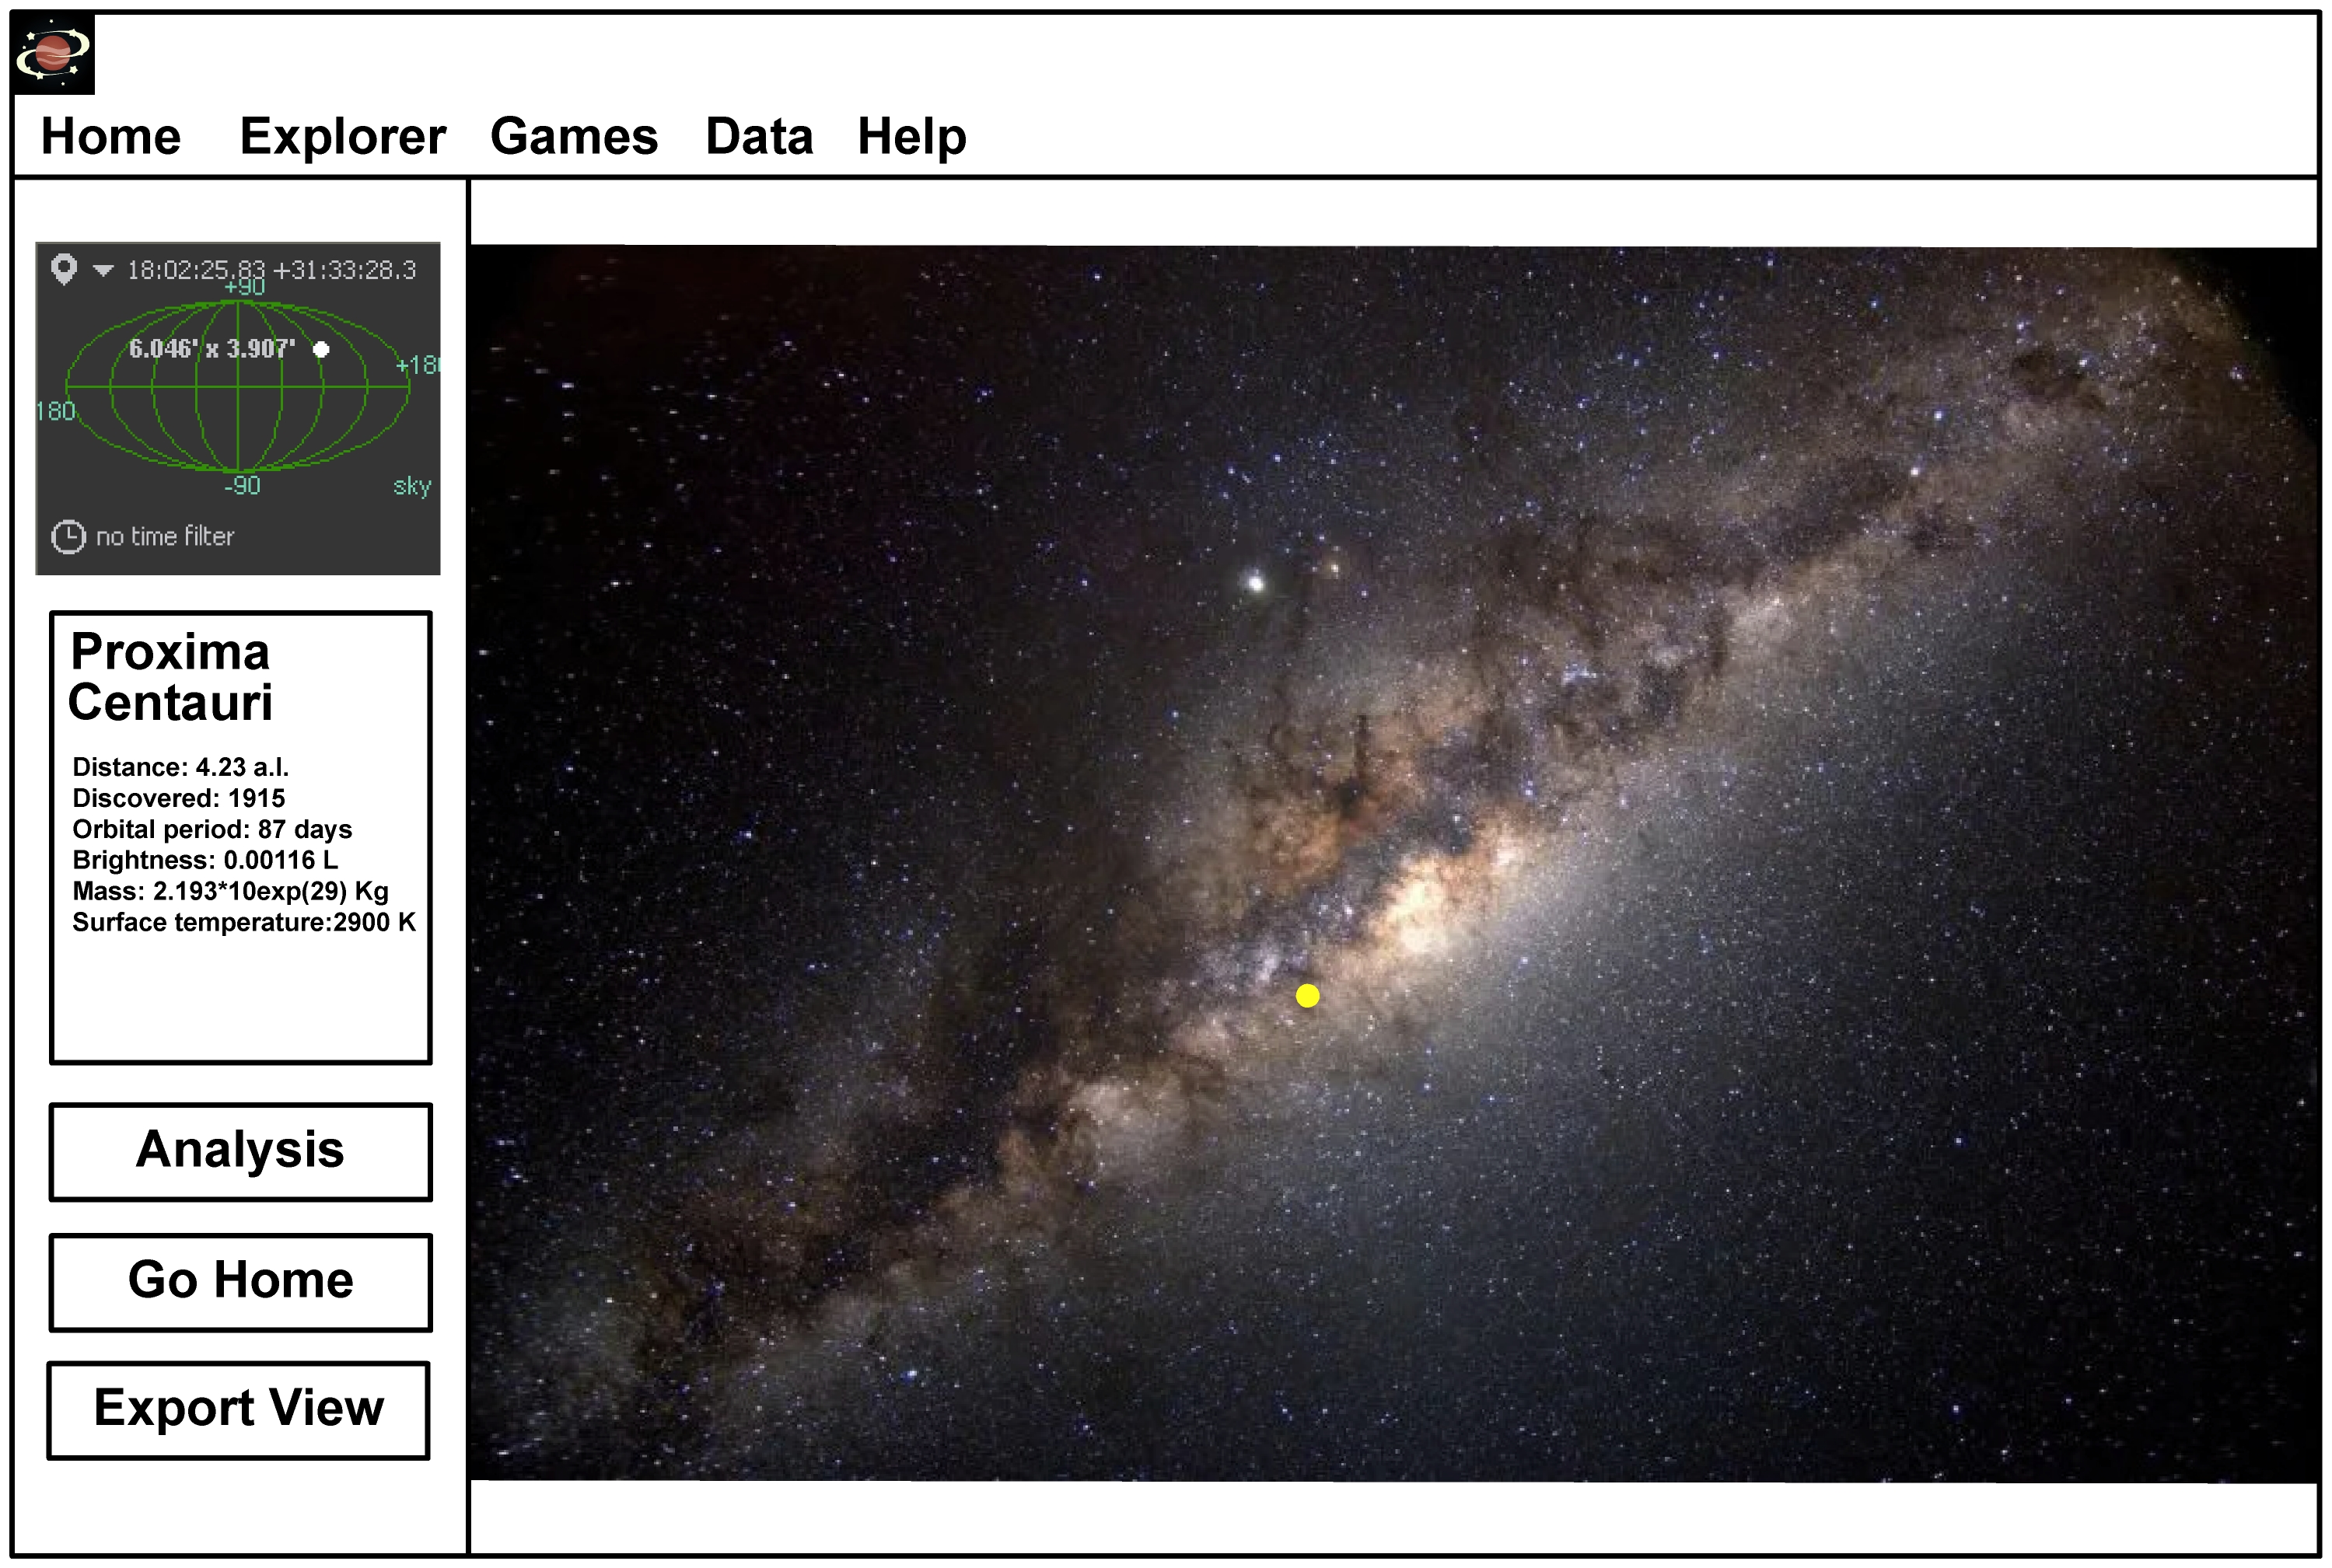
\includegraphics[width=\textwidth]{./img/explorer.jpg}
            \end{figure}

        \end{column}

    \end{columns}

\end{frame}

\begin{frame}{Interactive area}

    \begin{columns}[c, onlytextwidth]

        \begin{column}{0.7\textwidth}

            \begin{figure}[H]
                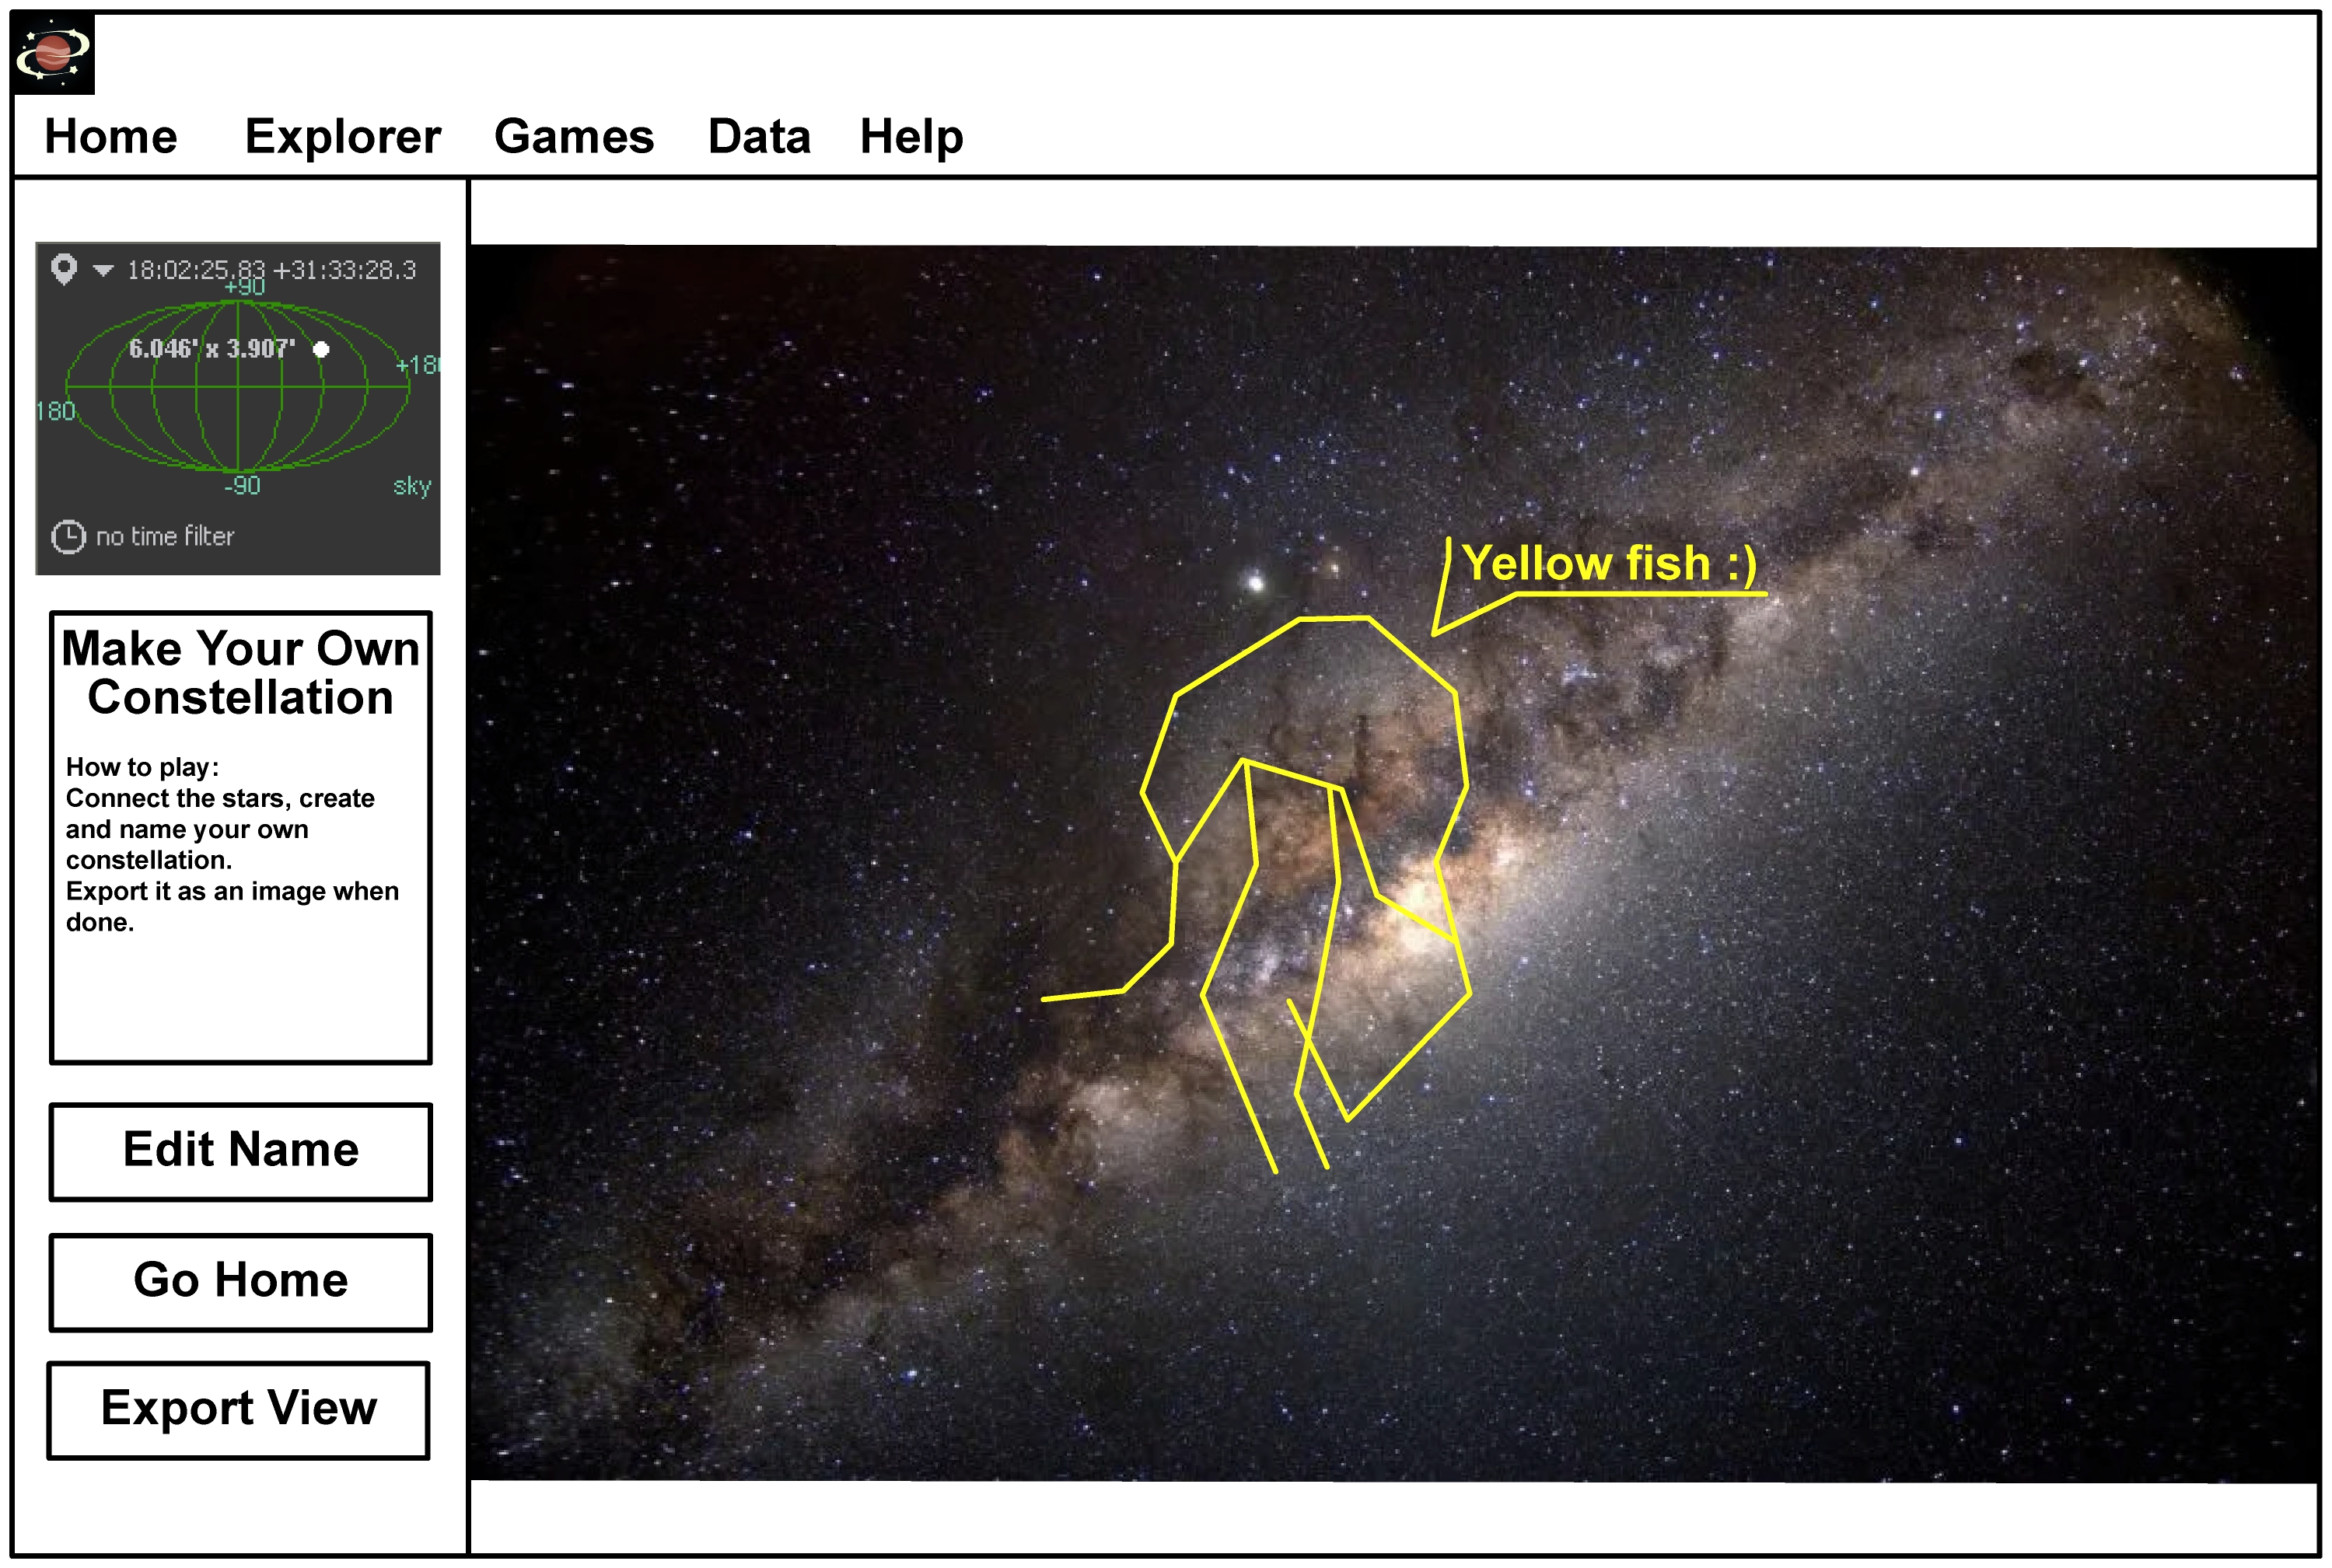
\includegraphics[width=\textwidth]{./img/games.jpg}
            \end{figure}

        \end{column}
        \hfill
        \begin{column}{0.28\textwidth}

            \begin{itemize}
                \item Playground area of the app for kids
                \item Allows them to interactive with the universe while learning about it
            \end{itemize}

        \end{column}

    \end{columns}

\end{frame}

\begin{frame}{Data analysis}

    \begin{columns}[c, onlytextwidth]

        \begin{column}{0.28\textwidth}

            \begin{itemize}
                \item Perform data analysis on celestial bodies
                \item Visualize data in a meaningful way
                \item Export the results
            \end{itemize}

        \end{column}
        \hfill
        \begin{column}{0.7\textwidth}

            \begin{figure}[H]
                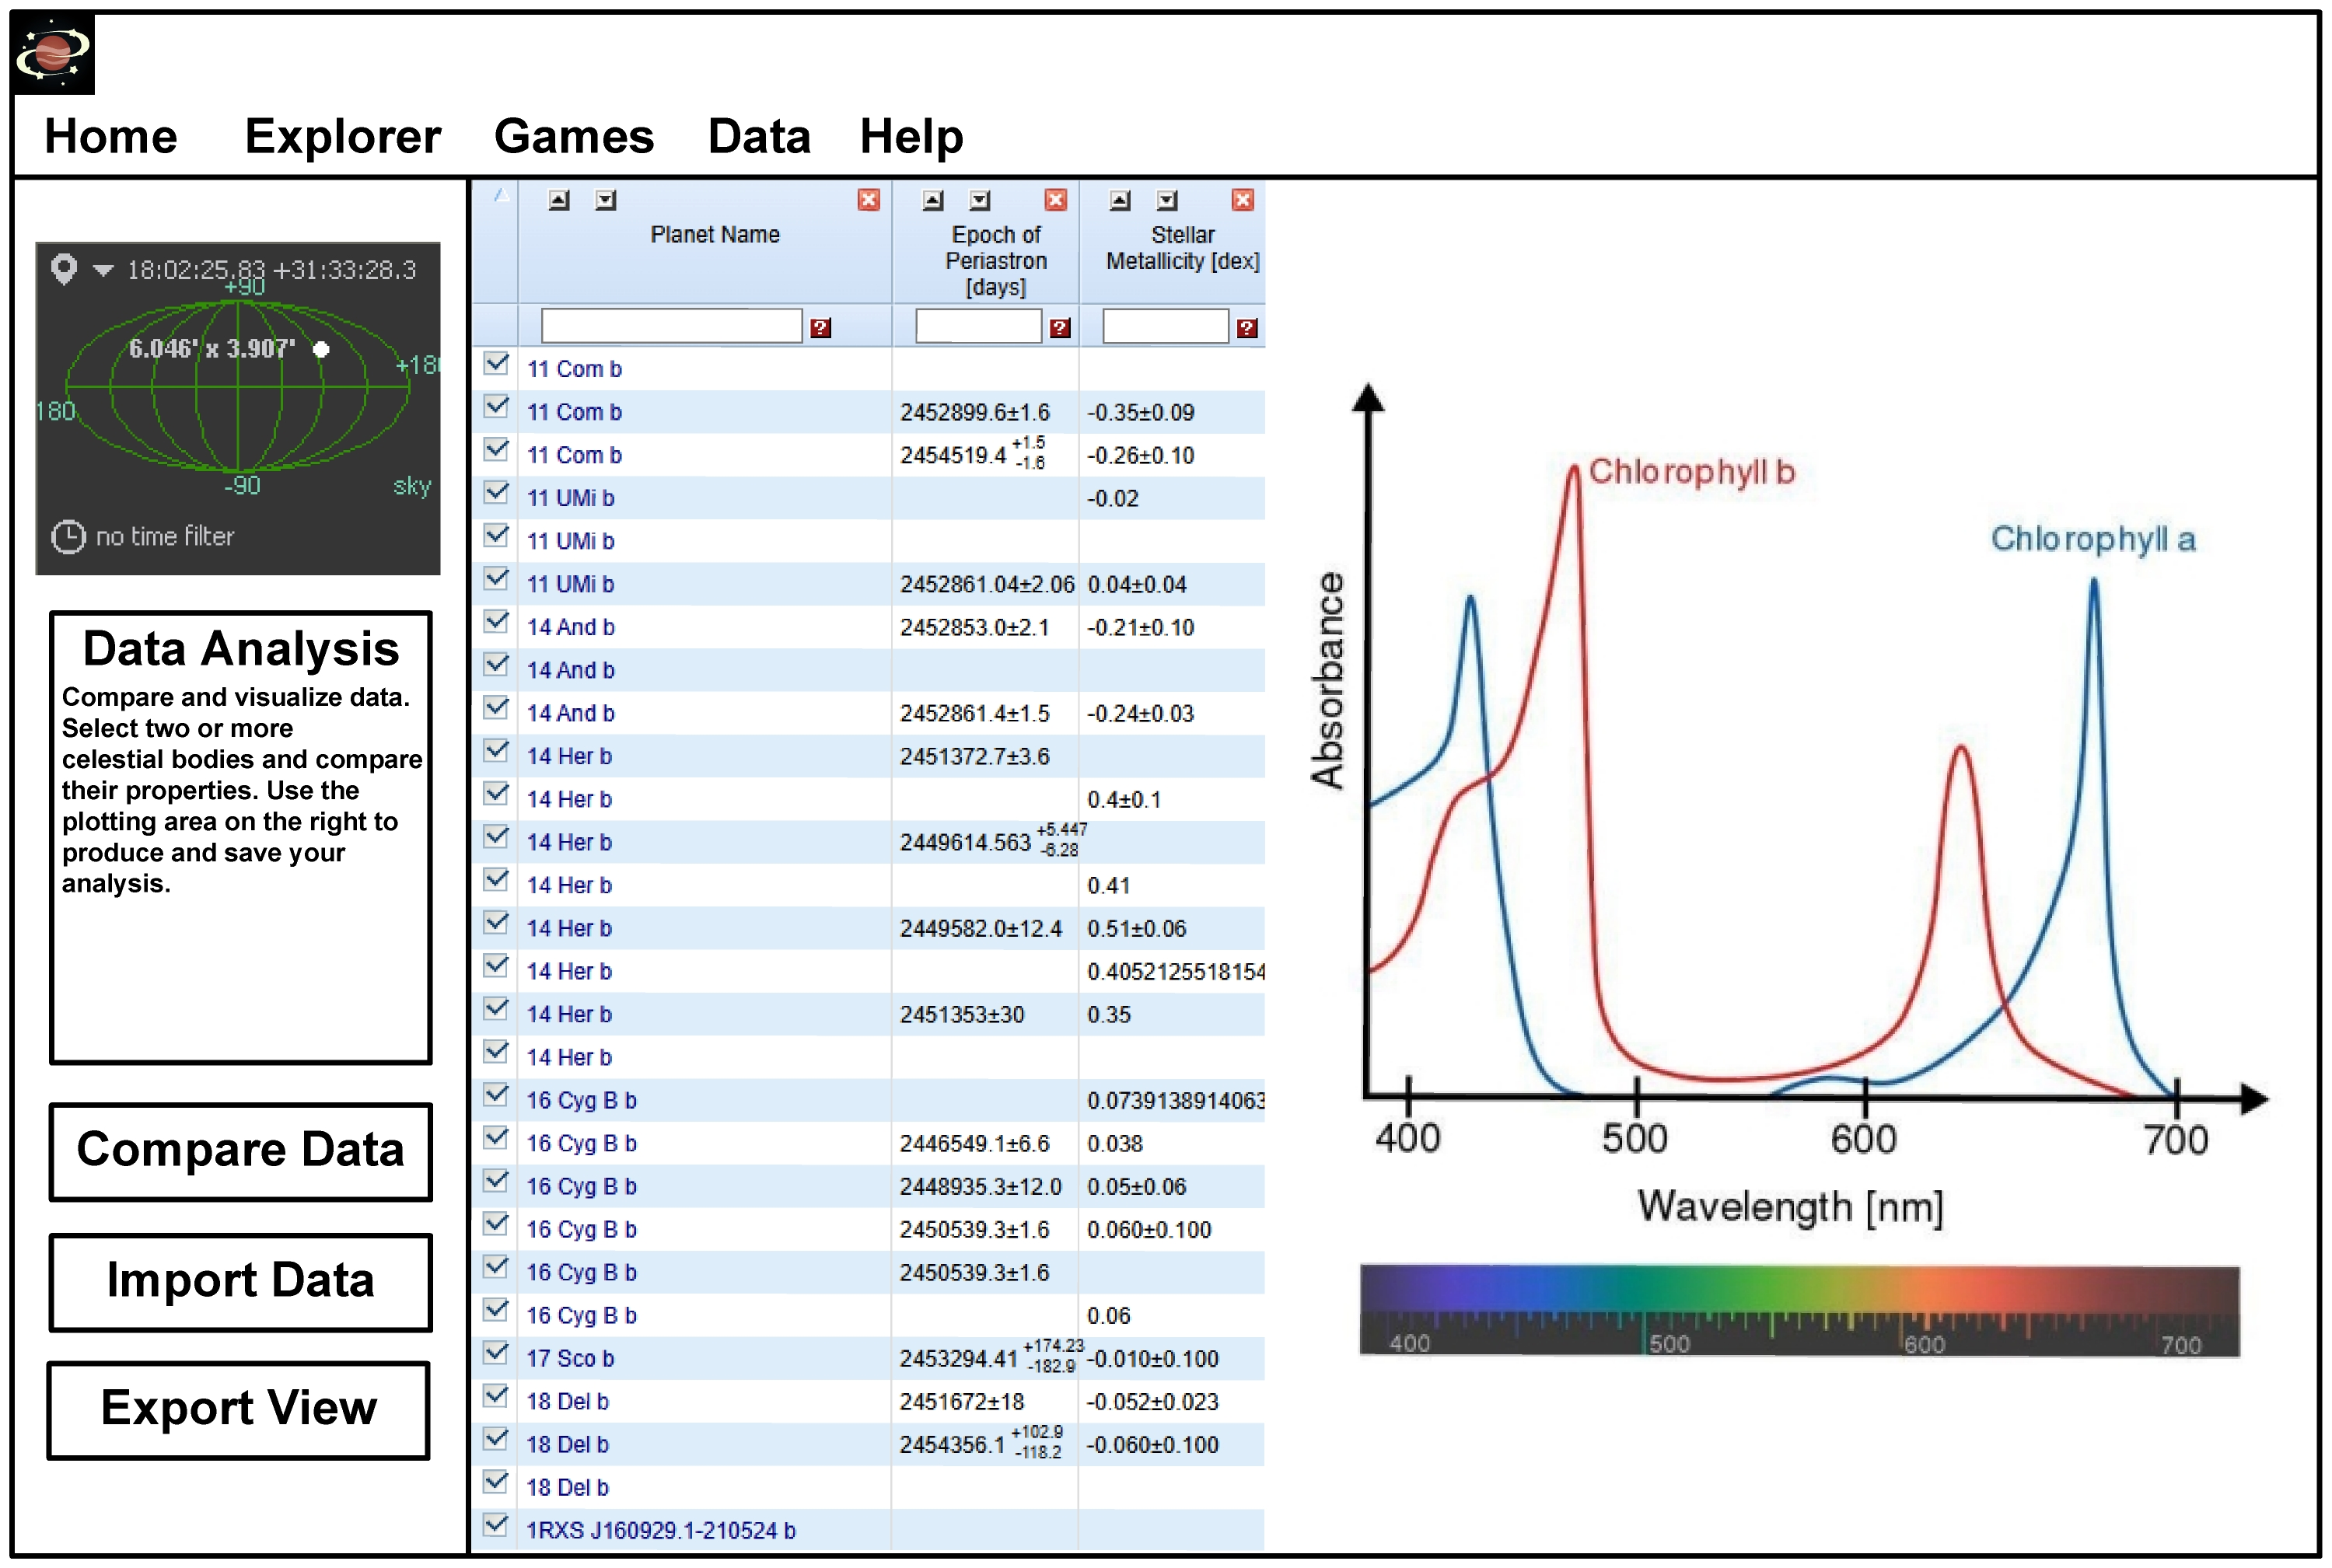
\includegraphics[width=\textwidth]{./img/data_analysis.jpg}
            \end{figure}

        \end{column}

    \end{columns}

\end{frame}

\begin{frame}{Possible developments}

    This project can be further developed by adding more entartaining features and educational content.

    \begin{itemize}
        \item Kids might be able to save their constellations and \textbf{share} them with friends
        \item A quiz section can be added to test the knowledge of the user
        \item On the home page, a daily fact about the progress of space exploration can be displayed
    \end{itemize}

\end{frame}

% References
\appendix
\begin{frame}[allowframebreaks]{References}
    \nocite{*}
    \bibliography{references}
\end{frame}

\end{document}